%!TEX root = main.tex

\chapter{Non-LTE Atmospheres}

% As we have discussed several times, LTE is a good
% approximation when the collisional rates for population and
% depopulation dominate the radiative rates and, as we have
% also mentioned, this is not the case when the density is
% low, the radiation density high, or the transition strong.
% In these cases, to obtain accurate results, we are forced to
% drop the assumption of LTE and adopt an non-LTE approach. By
% this, we mean that we calculate the population explicitly,
% taking into account the rate equations for the population
% and depopulation of a state -- by which we may mean either
% an ionization state or an excitation energy state.

% Treating a state in a non-LTE manner is computationally
% intensive, we are limited in the number of states that can
% be treated this way. For this reason, we normally chose
% adopt a non-LTE approach for the most important states and
% adopt LTE for the rest. Furthermore, even when we consider
% non-LTE distributions for ionization states and excitation
% states, the assumption of LTE for the particle velocities is
% still good. Thus, we can always assume the the particles
% have a Maxwellian distribution characterized by a single
% temperature $T$.
%
% \comment{How many lines are treated in non-LTE codes?}


In the approximation of LTE we assumed that all occupation numbers for
matter are given by the equilibrium values at the local temperature. The
extinction coefficient and the emissivity can then be calculated in a
straightforward manner using the techniques of
Chapter~\ref{chapter-lte-opacity-and-emissivity}, and this considerably
simplifies the solution of the equation of radiative transfer.

In this chapter we will consider the consequences of not adopting the
approximation of LTE and of instead calculating the ocupation numbers
for the excitation and ionization distributions using techniques from
statistical mechanics. The extinction coefficient and the emissivity
then follow from the ocupation numbers. However, we will continue to
assume the atmosphere is in steady state, we will continue to assume
that we have a static atmosphere in hydrostatic equilibrium, and we will
continue to assume that the distribution of massive particle velocities
is given by a Maxwellian at the local temperature. (An example of a
non-LTE problem in which we have to consider the time dependence
explicitly is the cooling and recombination region behind a
shock.)\comment{Need to explain somewhere why Maxwell is good even in
non-LTE conditions.}

\newslide

\section{Excitation Distribution}

The general LTE problem calculates both the excitation and ionization
distributions explicitly, without assuming that they are given by the
Boltzmann and Maxwell distributions. However, let us consider first a
special case of non-LTE problems, in which we will assume that the
ionization distribution is still given by the Saha distributions, and
investigate the implications of attempting to solve explicitly for the
excitation distribution. We will consider the more general case
subsequently.

In order to maintain a steady state on a macroscopic scale, we must have
statistical equilibrium, which means that the total rates of population
and depopulation of each level must be equal. Levels can be populated or
depopulated by either radiative or collisional processes. The radiative
processes we must consider are absorption and stimulated emission,
\begin{align}
\reversiblereaction{X&}{X' + \gamma},
\intertext{and spontaneous emission,}
\reaction{X + \gamma&}{X' + 2\gamma}.
\end{align}
In both, there is an exchange of between the internal energy of particle
$X$ or $X'$ and the photon. Recalling the definition of the Einstein
coefficients, the rate per unit volume of radiative transitions from
level $i$ to level $i'$ is
\begin{align}
n_i R_{ii'} \equiv 
\begin{cases}
n_i [A_{ii'} + B_{ii'} \int_0^\infty\!\!\!d\nu\:J_\nu(\nu) \psi(\nu)],&
\mbox{for desexcitations,}\\
n_i B_{ii'} \int_0^\infty\!\!\!d\nu\: J_\nu(\nu)\psi(\nu),&
\mbox{for excitations,}
\end{cases}
\end{align}
in which $n_i$ is the density of particles in level $i$.
The collisional processes we must consider are and collisional excitation
and de-excitation between states $X$ and $X'$,
\begin{align}
\reversiblereaction{X + Y&}{X' + Y},
\end{align}
Here there is an exchange between the internal energy of the ``target''
particle $X$ or $X'$ and and the kinetic energy of the ``colliding''
particle $Y$. The rate per unit volume of collisional transitions
between level $i$ and level $i'$ involving a colliding particle $Y$ is
\begin{align}
n_i n_Y C_{ii'} \equiv n_i n_Y \int_0^\infty\!\!\!dv_Y\: f_Y(v_Y) \sigma_{ii',Y}(v_Y) v_Y,
\end{align}
in which $v_Y$ is the speed of the colliding particle, $f_Y$ the
distribution function of speed, and $\sigma_{ii',Y}$ the differential
cross-section for the transition. We can write this as
\begin{align}
n_i n_Y C_{ii'} \equiv n_i n_Y \left<\sigma_{ii',Y} v_Y\right>,
\end{align}
in which $\left<\sigma_{ii',Y} v_Y\right>$ is the mean product of the
cross-section and the speed integrated over the distribution of speeds.

Possible colliding particles include electrons, ions, and neutral atoms.
Electrons always dominate ions, because although ions and electrons have
similar cross-sections, the mean speed of the electrons is
$(m_\mathrm{ion}/m_e)^{1/2} \approx 43 A_\mathrm{ion}^{1/2}$ larger than
that of the ions. Electrons often dominate collisions with neutral
atoms, both because neutral atoms are also much slower than electrons
and because the Coulomb force of an electron leads to a much higher
cross-section than the Van der Waals force of a neutral atom. However,
in very cool atmospheres, electrons can become very scarce, and
collisions with hydrogen atoms might become important. In what follows,
though, we will assume that electrons dominate collisions; including
collisions with hydrogen atoms modifies the details of the non-LTE
calculation, but does not change its essence.

In statistical equilibrium, the net rates of population and depopulation
of a level balance, and we have
\begin{align}
\sum_{i'\ne i} n_i (R_{ii'} + n_e C_{ii'}) = \sum_{i'\ne i} n_{i'} (R_{i'i} +
n_e C_{i'i}).
\end{align}
or, more concisely,
\begin{align}
\sum_{i'\ne i} \left[
n_i (R_{ii'} + n_e C_{ii'}) - n_{i'} (R_{i'i} + n_e C_{i'i})
\right] = 0.
\eqlabel{non-lte-excitation}
\end{align}
We can see straight away that we have one familiar and two new
complications:
\begin{enumerate}
\item 
The collisional coefficients $n_e C_{ii'}$ depend on the temperature and
electron density. More precisely, $C_{ii'}$ depends on the distribution
of velocities, but as we are still assuming that we have a Maxwell
distribution of velocities, this reduces to a dependence on temperature.
Thus, the excitation distribution depends on density and temperature.
This dependence also occurs in a different form in LTE.
\item 
The radiative coefficients $R_{ii'}$ depends on the mean specific
intensity $J_\nu$ at the frequencies $\nu_{ii'}$ given by $h\nu_{ii'} =
|E_i - E_i'|$. This tight coupling between matter and radiation is new.
In LTE, the interaction between matter and radiation is normally
required to satisfy radiative equilibrium (or more generally thermal
equilibrium), and this results in a much looser coupling through the
temperature.
\item 
The population of each state depends on the populations in all of the
states that can populate or depopulate that state. Again, this is not
present in LTE.
\end{enumerate}
Thus, non-LTE atmospheres have a local coupling between matter and
radiation, a local coupling between states, a local coupling involving
thermal equilibrium, and one non-local coupling from the transfer of
radiation, whereas LTE problems have only the latter two. The additional
tight local couplings make non-LTE atmospheres more difficult to
understand and to model than LTE atmospheres.

\newslide

\section{Excitation-Ionization Distribution}

Now let us relax the assumption that the ionization distribution is
given by the Saha distribution and consider the general non-LTE problem.
We now must consider not only processes that can change the excitation
state, but also those that can change the the ionization state. These
includes photoionization and spontaneous radiative recombination,
\begin{align}
\reversiblereaction{X^+ + e^-&}{X + \gamma},
\intertext{along with the stimulated radiative recombination,}
\reaction{X^+ + e^- + \gamma&}{X + 2\gamma},
\intertext{and collisional ionization and three-body collisional
recombination,}
\reversiblereaction{X^+ + 2e^-&}{X + e^-}.
\end{align}
If the density of state $i$ of ionization state $j$ is $n_{ij}$, the net
radiative and collisional rate coefficients for transitions from state
$ij$ to state $i'j$ (excitation and de-excitation) are $R_{ii'j}$ and
$n_e C_{ii'j}$, the net radiative and collision rate coefficientes for
transitions from state $ij$ to state $i'j+1$ (ionization) are
$R_{ii'j}^+$ and $n_e C_{ii'j}^+$, and the net radiative and collisional
rate coefficients for transitions from state $ij$ to state $i'j-1$
(recombination) are $n_eR_{ii'j}^-$ and $n_e^2C_{ii'j}^-$ the equation
of statistical equilibrium is
\begin{align}
&\sum_{i'\ne i} 
\left[n_{ij} (R_{ii'j} + n_e C_{ii'j}) 
-
 n_{i'j} (R_{i'ij} + n_e C_{i'ij})\right] + \\
&
\sum_{i'}      
\left[n_{ij} (R_{ii'j}^+ + n_e C_{ii'j}^+) 
-
n_{i'j+1} (n_e R_{i'ij+1}^- + n_e^2 C_{i'ij+1}^-)\right]+ \\
&\sum_{i'}      
\left[n_{ij} (n_e R_{ii'j}^- + n_e^2 C_{ii'j}^-)
-
n_{i'j-1} (R_{i'ij-1}^+ + n_e C_{i'ij-1}^+)\right]
= 0.
\end{align}
We can see that this introduces a yet more severe form of the tight
coupling that we had when we considered only the excitation
distribution. Now, each level is coupled to every excitation level of
every ionization state and matter is coupled to the radiation field at
any frequency that can produce a transition between any two excitation
levels of any two ionization states.

%\comment{Discuss autoionization and dielectronic recombination. Charge exchange?}

\newslide

\section{Recovering LTE}

The equations of statistical equilibrium, with their high degree of
coupling, are sufficiently awful that a natural reaction is to wonder if
assuming LTE is really \emph{that} bad. So let us consider under what
conditions LTE is likely to be a good approximation, and under what
conditions we need to worry about non-LTE effects.

We will once again begin by considering the restricted non-LTE problem
in which we solve explicitly only for the excitation distribution. In
perfect thermodynamic equilibrium we have detailed balance, so the
radiative and collisional transition rates between two states balance,
and we have
\begin{align}
n_i^*R_{ii'}^* &= n_{i'}^*R_{i'i}^*
\intertext{and}
n_i^*n_e^*C_{ii'}^* &= n_{i'}^*n_e^*C_{i'i}^*.
\end{align}
Recall that we use a superscript $*$ for quantities in thermodynamic
equilibrium. Summing over all states gives
\begin{align}
\sum_{i'\ne i}n_i^*R_{ii'}^* &= \sum_{i'\ne i}n_{i'}^*R_{i'i}^*
\intertext{and}
\sum_{i'\ne i}n_i^*n_e^*C_{ii'}^* &= \sum_{i'\ne i}n_{i'}^*n_e^*C_{i'i}^*.
\end{align}
Multiplying the second of these by $n_e/n_e^*$ and adding we obtain,
\begin{align}
\sum_{i'\ne i} n_i (R_{ii'} + n_e C_{ii'}) = \sum_{i'\ne i} n_{i'} (R_{i'i} +
n_e C_{i'i})\\
\sum_{i'\ne i} n_i^* (R_{ii'}^* + n_e C_{ii'}^*) = \sum_{i'\ne i}
n_{i'}^* (R_{i'i}^* + n_e C_{i'i}^*).
\end{align}
Comparing this to \eqref{non-lte-excitation}, the equation for
statistical equilibrium, we see that LTE will be good approximation, and
we will have $n_i \approx n_i^*$, to the extent that
\begin{align}
R_{ii'} + n_e C_{ii'} \approx R_{ii'}^* + n_e C_{ii'}^*
\eqlabel{lte-rate}
\end{align}
is a good approximation. Let's consider $C_{ii'}$. This will be the
result of integrating a differential cross-section for excitation or
de-excitation over the distribution of electron velocities. The
distribution of velocities is still given by a Maxwell distribution, and
so
\begin{align}
C_{ii'} = C_{ii'}^*.
\end{align}
Armed with this, we see that \eqref{lte-rate} reduces to
\begin{align}
R_{ii'} + n_e C_{ii'}^* \approx R_{ii'}^* + n_e C_{ii'}^*.
\eqlabel{lte-is-good}
\end{align}
This is a good approximation when either $R_{ii'} \approx R_{ii'}^*$ or
both $R_{ii'} \ll n_e C_{ii'}$ and $R_{ii'}^* \ll n_e C_{ii'}$. Since
the radiative rate coefficient $R_{ii'}$ depends on $J_\nu$, the first
case corresponds to $J_\nu \approx B_\nu$. The second case corresponds
to collisions being dominant both in thermal equilibrium and in the
conditions being considered.

We can apply exactly the same arguments to the general non-LTE case in
which we solve for both the excitation and ionization distribution. Once
again, we discover that LTE is a good approximation when either $J_\nu
\approx B_\nu$ or when collisions are dominant.

Looking back to section~\ref{section:diffusion-approximation}, we can
now justify using LTE in the diffusion approximation for the transfer of
radiation in the interior of a star. The density and temperatures are
high, which tends to make collisions dominant, and furthermore $J_\nu
\approx B_\nu$. We satisfy both of our criterion for LTE being a good
approximation.

However, we can now see that LTE will \emph{never} be a truely good
approximation in an atmosphere. Here, the $J_\nu$ departs significantly
from $B_\nu$, because of the temperature gradients and the presense of
the outer boundary, and the densities are low enough that radiative
transition rates become important for suffiently strong lines. We might
think that if only a few transitions in an atom fail to satisfy the
conditions for LTE, we can still treat the other levels as is they
satisfied LTE. Unfortunately, because of the coupling between levels in
non-LTE problems, this is dangerous; it only needs one transition to
fail to satisfy the conditions for LTE to perturb an entire atom or
species out of LTE.

On the other hand, we can at least identify those situations in which
LTE is a worse approximation. These will be those in which the radiation
field is far from Planckian and in which radiative rates are not
negligible compared to collisional rates. As we have just mentioned,
being in an atmosphere, or more generally outside of the optically thick
interior, guarantees that there are significant departures from
Planckian radiation. Furthermore, high effective temperatures (higher
$J_\nu$ and hence higher radiative rates), strong lines (higher
radiative rates), and lower densities (lower collisional rates) all
conspire to make LTE a worse approximation. We can then see that we
should be most suspicious of LTE in winds, in the atmospheres of hot
stars, and in the atmospheres of supergiant stars. Conversely, we might
expect LTE to be a reasonable approximation in dwarf or degenerate stars
and in cool stars.

%
%
%An astrophysically interesting question is whether LTE might apply in
%coronal conditions, in which the density of both electrons and photons
%is low. The low density will act reduce the rate of collisions,
%stimulated radiative processes, and absorptive radiative processes, but
%spontaneous radiative processes continue unhindered. For example, the
%ionization balance will be set essentially by the competition between
%collisional ionization and radiative recombination. Thus, the radiative
%rates are important, and LTE is a poor approximation. ({Similar
%arguments hold in the interstellar medium, where the density is even
%lower and the radiation field even more dilute. Spontaneous emission and
%radiative recombination can still be important, and LTE is often a
%spectacularly bad approximation.)
%
%Of course, much depends on the degree of accuracy we demand; if we only
%want a rough continuum shape, LTE is probably adequate everywhere except
%in the extreme ultraviolet region of O stars, but if we want to
%determine precise line profiles, LTE is probably inadequate to some
%degree even in cool dwarfs.
%
%\section{Two-Level Atom Without Continuum}
%
%\begin{figure}
%\begin{center}
%%\input{Figures/two-level-atom.tex}
%\end{center}
%\caption{The two-level atom without continuum, showing the collsional
%and radiative transitions that control the level populations.}
%\label{figure-two-level-atom}
%\end{figure}
%
%
%We can gain an understanding of non-LTE effects by considering a simple
%model for a two-level atom without continuum opacity. The atom has two
%states, 0 and 1, with state 0 being the ground state and state 1 having
%an excitation energy of $E$. The states are populated and depopulated by
%radiative and collisional transitions, as shown in
%Figure~\ref{figure-two-level-atom}. This system is complex enough to
%show interesting non-LTE effects, but simple enough that we can generate
%relatively simple explanations for these effects.
%
%We will want to determine the source function. The emission coefficient
%is
%\begin{align}
%\eta_\nu(\nu) = \frac{1}{4\pi} n_1 A_{10} h\nu \psi_\nu(\nu),
%\end{align}
%and the absorption coefficient is
%\begin{align}
%\kappa_\nu(\nu) = \frac{1}{4\pi} (n_0 B_{01} - n_1 B_{10}) h\nu \phi_\nu(\nu).
%\end{align}
%Then, the source function is then given by
%\begin{align}
%S_\nu(\nu) \equiv \frac{\eta_\nu(\nu)}{\kappa_\nu(\nu)} 
%= \frac{n_1 A_{10}}{n_0 B_{01} - n_1 B_{10}} \frac{\psi_\nu(\nu)}{\phi_\nu(\nu)}.
%\end{align}
%If we have complete redistribution, then $\phi_\nu =
%\psi_\nu$ and we have
%\begin{align}
%S_\nu(\nu) = \frac{n_1 A_{10}}{n_0 B_{01} - n_1 B_{10}} \equiv S^L.
%\eqlabel{two-level-atom-a}
%\end{align}
%We now need to determine the populations $n_0$ and $n_1$
%from the rate equation
%\begin{align}
%n_0(R_{01} + n_e C_{01}) = n_1(R_{10} + n_e C_{10}).
%\eqlabel{two-level-atom-b}
%\end{align}
%We know from the definition of the Einstein coefficients
%that
%\begin{align}
%R_{01} &= B_{01} \int_0^\infty\!\!\!d\nu\: J_\nu(\nu)\phi_\nu(\nu)
%\equiv B_{01}\bar J_\nu
%\eqlabel{two-level-atom-c}
%\intertext{and}
%R_{10} &=  A_{10} + B_{10} \int_0^\infty\!\!\!d\nu\: J_\nu(\nu)\psi_\nu(\nu)
%= A_{10} + B_{10}\bar J_\nu.
%\eqlabel{two-level-atom-d}
%\end{align}
%We now need to consider the collisional rates. In
%thermodynamic equilbrium, we have detailed balance, and so
%\begin{align}
%n_0^* n_e^* C_{01}^* = n_1^* n_e^* C_{10}^*,
%\end{align}
%in which, as usual, the $*$ indicates a value in thermodynamic
%equilibrium. As above, $C_{01} = C_{01}^*$, as we are integrating a
%cross-section over a Maxwellian, and so $C_{01}$ depends only on the
%temperature. Thus, we have
%\begin{align}
%\frac{C_{10}}{C_{01}} = 
%\frac{C_{10}^*}{C_{01}^*} = 
%\frac{n_0^*}{n_1^*} =
%\frac{g_0}{g_1} \exp E/kT.
%\eqlabel{two-level-atom-e}
%\end{align}
%Combining Equations (\ref{equation-two-level-atom-a}),
%(\ref{equation-two-level-atom-b}), (\ref{equation-two-level-atom-c}),
%(\ref{equation-two-level-atom-d}), and
%(\ref{equation-two-level-atom-e}), and using the Einstein relations
%between the Einstein coefficients, we obtain
%\begin{align}
%S^L = (1 - \varepsilon) \bar J_\nu + \varepsilon B_\nu,
%\label{equation-two-level-atom-source-function}
%\end{align}
%in which 
%\begin{align}
%\varepsilon \equiv \frac{\varepsilon'}{1 + \varepsilon'}
%\end{align}
%and 
%\begin{align}
%\varepsilon' \equiv \frac{n_e C_{10}}{A_{10}} (1 - e^{-E/kT}).
%\end{align}
%
%\comment{Use this to show that LTE is inconsistent. If
%$S_\nu = B_\nu$, then at the surface $J_\nu = B_\nu/2$,
%so $S_\nu = (1+\varepsilon)B_\nu/2$, which is only equal to
%$B_\nu$ if $\varepsilon=1$.}
%
%We can see straight away how the balance between collisional and
%radiative transitions leads to departures from the LTE. If collisional
%transitions dominate radiative transitions, then $n_e C_{10}/A_{10}
%\rightarrow
%\infty$, $\varepsilon' \rightarrow \infty$, $\varepsilon
%\rightarrow 1$, and $S^L \rightarrow B_\nu$, and we recover the the LTE limit.
%However, as radiative transitions become more important, $n_e
%C_{10}/A_{10} \rightarrow 0$, $\varepsilon'$ becomes smaller,
%$\varepsilon$ becomes closer to zero, and $S^L$ deviates from $B_\nu$.
%In the limit that radiative transitions dominate, $\varepsilon'
%\rightarrow 0$, $\varepsilon \rightarrow 0$, and $S^L \rightarrow \bar
%J_\nu$. In this case, we only recover LTE if $\bar J_\nu \approx B_\nu$.
%
%\begin{figure}
%\begin{center}
%\vspace{1in}
%$S_\nu$ against $\tau^L$ for the two-level atom without continuum.
%\vspace{1in}
%\end{center}
%\caption{The source function for the two-level atom without continuum.}
%\label{figure-two-level-atom-source-function}
%\end{figure}
%
%We can solve for the source function numerically, obtaining the results
%shown in Figure~\ref{figure-two-level-atom-source-function} for an
%atmosphere in which $B_\nu$, $\phi_\nu$, and $\varepsilon$ are constant.
%This figure shows the source function $S^L$ against the integrated line
%opacity defined by 
%\begin{align}
%\frac{d\tau^L}{dz} 
%= -\int_0^\infty\!\!\!d\nu\: \alpha_\nu
%= -\int_0^\infty\!\!\!d\nu\: \alpha^L \phi_\nu
%= -\alpha^L.
%\end{align}
%The solution shows three interesting characteristics:
%
%\begin{enumerate}
%
%\item
%At depth, the source function $S_\nu$ approaches the local
%Planck function $B_\nu$.
%
%\item
%The surface source function $S_\nu(0)$ is not give by the
%surface Planck function $B_\nu(0)$ but by $S_\nu(0) =
%\varepsilon^{1/2} B_\nu(0)$. This result is independent of
%$\phi_\nu$.
%
%\item
%The optical depth below which we have $S_\nu \approx B_\nu$
%depends on $\varepsilon$ and $\phi_\nu$. This optical depth
%is known as the thermalization depth, because radiation that
%arises from a source with $S_\nu = B_\nu$ is known as
%thermal radiation. The thermalization depth is traditionally
%denoted $\Lambda$, but should not be confused with the
%$\Lambda$-operator (which was defined by $J_\nu \equiv
%\Lambda(S_\nu)$). The value of the thermalization depth
%$\Lambda$ depends on both $\varepsilon$ and $\phi_\nu$. For
%a Gaussian profile we have
%\begin{align}
%\Lambda \sim \frac{1}{\varepsilon},
%\end{align}
%for a Lorentzian profile 
%\begin{align}
%\Lambda \sim \frac{1}{\varepsilon^2},
%\end{align}
%and for a Voigt profile
%\begin{align}
%\Lambda \sim \frac{a}{\varepsilon^2},
%\end{align}
%in which $a = \Gamma / 4 \pi \Delta\nu_\mathrm{D}$. (This
%approximation is only valid for $a \ll 1$, but this is
%normally the case.)
%
%\end{enumerate}
%
%% We can see that if collisions dominate, $\varepsilon
%% \rightarrow 1$, $S_\nu(0) \rightarrow B_\nu(0)$, so $S_\nu$
%% is equal to the local Planck function both at depth and at
%% the surface, and we recover the LTE approximation for the
%% source function. (Putting $\varepsilon$ into the expressions
%% given above for the thermalization depth does not work, as
%% these expression neglect terms of order unity. The real
%% thermalization depth tends to zero as $\varepsilon$ tends to
%% 1.)
%
%% However, in general, collisions will not completely dominate and the
%% source function near the surface will be lower than the local Planck
%% function. This is a clear deviation from the behaviour of the source
%% function in the LTE approximation.
%
%% At depth, though, we still have $S_\nu \approx B_\nu$. This is because
%% at depth $J_\nu \rightarrow B_\nu$ and both radiative and collisional
%% transitions will act to produce a thermal equilibrium distribution of
%% state populations. In this case, LTE is a good approximation and so
%% $S_\nu
%% \rightarrow B_\nu$.
%
%Let's try to understand these results one by one. At depth the diffusion
%approximation will be valid and we will have $J_\nu \approx S_\nu$ or,
%in the notation of this problem, $\bar J_\nu = S^L$. Substituting this
%result into Equation~(\ref{equation-two-level-atom-source-function}), the
%equation for $S^L$ in terms of $\bar J_\nu$, leads to
%\begin{align}
%S^L &= (1 - \varepsilon) S^L + \varepsilon B_\nu,
%\intertext{which has the solution}
%S^L &= B_\nu.
%\end{align}
%
%Close to the surface at $\tau^L = 0$, photons can escape and $\bar
%J_\nu$ will drop below $B_\nu$. To see this, first let's assume that
%$\bar J_\nu$ does not drop below $B_\nu$ close to the surface, and so
%$S^L = B_\nu$ throughout the atmosphere. In this case, we can use the
%Eddington-Barbier relation to show that $\bar J_\nu = B_\nu/2$ at the
%surface, which implies that $S^L = (1 - \varepsilon/2) B_\nu$ at
%surface. However, this contradicts our assumption that $S^L = B_\nu$.
%Self-consistency can only attained if $\bar J_\nu$ and hence $S^L$ drop
%below $B_\nu$ as we approach the surface. (Proving that $S^L(0) =
%\varepsilon^{1/2} B_\nu$ is more tricky. See Ivanov (1973), Rybycki
%(1984), and Hubeny (1987).)
%
%One consequence of $\bar J$ and hence $S^L$ dropping below $B_\nu$ is
%the depopulation of the upper level relative to LTE. We can see this as
%follows. We write the source function as
%\begin{align}
%S^L 
%= \frac{j^L}{\alpha^L}
%= \frac{n_1 A_{10}}{n_0 B_{01} - n_1 B_{10}}.
%\end{align}
%This can be rearranged to give the ratio of level populations $n_1/n_0$
%in terms of the Einstein coefficients and the source function,
%\begin{align}
%\frac{n_1}{n_0}
%= \frac{B_{01}}{A_{10}/S^L + B_{10}}.
%\label{equation-n1-n0-S}
%\end{align}
%In LTE, we have $S^L = B_\nu$, $n_1 = n_1^*$, and $n_0 = n_0^*$, hence
%\begin{align}
%\frac{n_1^*}{n_0^*}
%= \frac{B_{01}}{A_{10}/B_\nu + B_{10}}.
%\label{equation-n1-n0-B}
%\end{align}
%Comparing Equations~(\ref{equation-n1-n0-S}) and
%(\ref{equation-n1-n0-B}), we see that if $S^L < B_nu$, then
%\begin{align}
%\frac{n_1}{n_0}
%< 
%\frac{n_1^*}{n_0^*}.
%\end{align}
%Thus, the non-LTE effects near the surface imply a depopulation of the
%upper level. We can understand this depopulation from the rate
%equations. Let's consider the extreme case in which $\bar J_\nu = 0$.
%Here, collisional transitions and spontaneous emissions continue at the
%same rate, but absorptions and spontaneous emissions are suppressed.
%Compared to LTE, the result is a net loss of transitions that populate
%the upper level, since in LTE there are more absorptions than
%spontaneous emissions. The populations will adjust to this by reducing
%the fraction in the upper state. Intermediate cases, with $0 < \bar
%J_\nu < B_\nu$, are similar.
%
%Understanding the values of $S^L$ at the surface and at depth is thus
%relatively straightforward. The puzzle is why the effects of the
%surface, which causes $S^L$ to be smaller than $B_\nu$, reaches so far
%into the atmosphere. We might expect the surface to reach only one mean
%free path for an average photon to $\tau^L
%\approx 1$. However, for a typical line with a Lorentzian
%profile and $\varepsilon
%\approx 10^{-6}$, the effects of the surface is seen to an
%optical depth of roughly $\tau^L \approx 10^{12}$!
%
%The answer comes from considering the transfer of line
%radiation more closely. First, we must note that the optical
%depth used here and above is the integrated line optical
%depth defined by
%\begin{align}
%\tau^L = \int_0^z\!\!\!dz\: \alpha^L.
%\end{align}
%The real optical depth depends on the frequency and the line
%profile:
%\begin{align}
%\tau_\nu 
%= \int_0^z\!\!\!dz\: \alpha_\nu
%= \int_0^z\!\!\!dz\: \alpha^L \phi_\nu
%= \tau^L \phi_\nu.
%\end{align}
%Thus, the real opacity and real optical depth depend on
%where we are in the line: in the line core, where $\phi_\nu
%\sim 1$, the opacity and optical depth will be high, but in
%the line wings, where $\phi_\nu \ll 1$, they can be much
%lower.
%
%\begin{figure}
%\begin{center}
%%\input{FIGURES/random-walk-flowchart.tex}
%\end{center}
%\caption{A flow-chart showing the transfer of photons in the escaped
%probability approximation.}
%\label{random-walk-flowchart}
%\end{figure}
%
%Now lets consider what happens when a line photon is emitted deep in the
%atmosphere, but for the moment assuming that all photons are emitted in
%the line core, as is most probable. The photon is emitted in the line
%core and so will travel $\Delta\tau^L \sim 1$ before being absorbed and
%exciting an electron from the 0 level to 1 level. This excited electron
%will then either decay collisionally. If it decays collisionally,
%nothing further happens: the photon is destroyed. If it decays
%radiatively, another photon will be emitted in the line core and will
%travel another $\Delta\tau^L \sim 1$ before being absorbed. This process
%will continue until the photon is absorbed and destroyed by a
%collisional de-excitation. Recall that we interpreted $\varepsilon$ as a
%destruction probability; thus, the photon will be absorbed and
%re-emitted on average $1/P_\mathrm{d}$ times before being finally
%destroyed. Thus, the line photons will perform a random walk with a RMS
%displacement of $P_\mathrm{d}^{-1/2}$, but this is just
%$\varepsilon^{-1/2}$. This result is interesting, in that it is larger
%than the 1 optical depth we obtain when photons are immediately recycled
%into the thermal pool. However, by itself it would indicate that
%$\Lambda \sim 1/\varepsilon^{-1/2}$, which is far lower than the real
%values of $\Lambda$.
%
%To better understand $\varepsilon$, let us define the photon
%destruction probability $P_\mathrm{d}$ as the probability
%that an excitation results in a collisional de-excitation.
%\begin{align}
%P_\mathrm{d} = \frac{n_e C_{10}}{A_{10} + n_e C_{10}} 
%\end{align}
%The two-level atom without continuum is an adequate
%approximation for UV resonance lines, which have $E \gg kT$,
%and so
%\begin{align}
%P_\mathrm{d} \approx \varepsilon.
%\end{align}
%Thus, $\varepsilon$ measures the relative importance of
%collisional and radiative transitions. We'll return to the
%concept of a destruction probability below.
%
%\comment{FIGURE: random walk with excursions to the wings.}
%
%We'll now lift the assumption that photons are always
%emitted in the core. When a photon is emitted in the wing,
%the opacity is low compared to the core and so although on
%average it still travels only one \emph{real} optical depth
%$\Delta\tau_\nu \sim 1$, this can correspond to many
%\emph{integrated} optical depths $\Delta\tau^L$. The principal
%escape mechanism now becomes an emission in the wings of the
%line followed by a transfer over a large distance. In a
%sense, the photons that escape are not the \emph{average}
%photons in the line core, but those few that make an
%excursion to the line wing. Thus, allowing excursions to the
%line wing can greatly increase the thermalization depth.
%
%Let's consider this in more detail in terms of the
%\emph{escape probablility approximation}. This approximation
%reduces all of radiative transfer to a simple concept: a
%photon is emitted, and either it escapes from the atmosphere
%or is immediately reabsorbed. This is not such a bad
%approximation for the case at hand: the majority of photons
%will be emitted in the line core and will be absorbed very
%close to their point of emission.
%
%We define the escape probability $P_\mathrm{e}(\tau^L)$ as the
%angle-averaged probability that a photon emitted at a
%certain optical depth will escape from the atmosphere. For a
%photon emitted at an angle $\mu$ and frequency $\mu$, the
%probability of escape is $e^{-\tau_\nu/\mu}$, where
%$\tau_\nu = \tau^L\phi_\nu$. Furthermore, the probability
%density function of the emission frequency is just
%$\phi_\nu$. Thus, averaging over angles and frequencies gives
%\begin{align}
%P_\mathrm{e}(\tau^L) &= \frac{1}{2}
%\int_0^1\!\!\!d\mu\int_0^\infty\!\!\!d\nu\:
%\phi_\nu(\nu)e^{-\tau^L\phi_\nu(\nu)/\mu}\\
%&=
%\frac{1}{2}
%\int_0^\infty\!\!\!d\nu\:
%\phi_\nu E_2(\tau^L\phi_\nu).
%\end{align}
%
%The thermalization depth corresponds to the maximum depth
%from which photons can escape. Thus, once emitted, a photon
%will have be absorbed and remitted $1/P_\mathrm{d}$ times,
%and each time it is emitted it has a probability
%$P_\mathrm{e}$ of escaping, so the combined escape
%probaility will be something like
%$P_\mathrm{e}/P_\mathrm{d}$. Now, if $P_\mathrm{e} \ll
%P_\mathrm{d}$, the combined probability of scale is low and
%there is a local coupling between the radiation field and
%matter. Thus, we expect LTE conditions to hold. On the other
%hand, if $P_\mathrm{e} \gg P_\mathrm{d}$, photons are more
%likely to escape than to be reabsorbed, and there is very
%weak local coupling between radiation and matter, and
%non-LTE conditions will prevail. Thus, it makes sense to
%define the thermalization depth $\Lambda$ as the point at
%which $P_\mathrm{e}(\tau^L) = P_\mathrm{d}$. Once we do
%this, we have an implicit equation for $\Lambda$,
%specifically,
%\begin{align}
%\frac{1}{2}
%\int_0^\infty\!\!\!d\nu\:
%\phi_\nu E_2(\Lambda\phi_\nu) =  P_\mathrm{d}.
%\end{align}
%If we substitute for $\phi_\nu$ in this equation and use
%$P_\mathrm{d} \approx \varepsilon$, we obtain the
%dependences of $\Lambda$ on $\varepsilon$ quoted above.
%
%\comment{Better to say that if $P_d = P_e$ than a photon has
%an equal chance of escape or destruction at each
%interaction, so half of the photons escape.}
%
%\comment{First-order escape theory gets $S(0)$ wrong;
%discuss second-order theory -- see Hubeny.}
%
%\section{Non-LTE Models}
%
%Non-LTE models have focused on O stars, as non-LTE effects
%are vitaly important here on account of the strong radiation
%fields and low densities in the extended winds.
%
%\comment{Mention Generation 0: the TLA and TLA+continuum
%work in the 1960s.}
%
%\comment{Also mention models for Ca in Sun.}
%
%Non-LTE model atmospheres are significantly more difficult
%to construct that LTE model atmospheres. In an LTE
%atmosphere, the entire state of matter at each point is
%represented by two themodynamic state variables, normally
%density and temperature. In a non-LTE atmosphere, we have
%the populations (or departure coefficients $b \equiv n/n^*$)
%for each level for which we relax the assumption of LTE.
%Progress in the field has therefore depended on a succession
%of improvements in numerical techniques.
%
%The earliest non-LTE models with the H and He models for hot
%stars constructed by Auer and Mihalas in the 1970s and used
%a method known as complete linearization to solve for the
%level populations. Unfortunately, this method was restricted
%to 10--15 levels and about 100 frequency points, which
%restricted it to H and He. Despite this restriction, the
%codes were enough to show important differences from LTE
%models, and this stimulated the study of non-LTE effects in
%general.
%
%During the 1970s, LTE line-blanketed models became mature,
%and were epitomized by the Kurucz models. Recall that these
%are LTE models in which lines are included in the
%determination of the structure of the atmosphere. The LTE
%line-blanketed modeld showed important distinctions from LTE
%non-blanketed models. In a sense then, at the beginning of
%the 1980s, one had the choice of two inadequate models for
%stars in which LTE effects are important: line-blanketed
%models without non-LTE effects or LTE-models without line
%blanketing.
%
%To rectify this great efforts were made in the 1980s to
%include other sources of opacity. The breakthrough was the
%development of a method known as the accelerated
%$\Lambda$-iteration. This allowed the treatment of of order
%100 levels and 1000 frequencies, which is enough to
%incorporate the light elements, C, N, O, and Si, which make
%significant contributions to the opacity. The most famous
%models in this category are those of Kudritzski's group.
%
%Nevertheless, with only 100 levels it is impossibly to
%directly incorporate iron-peak elements, such as Fe and Ni,
%as each element has hundreds of levels (the number of levels
%rises rapidly with the number of electrons). Thus, during
%the 1990s the focus became approximate methods for
%incorporating these into a non-LTE framework. The basic idea
%was to use ``super-levels'': these are groups of levels that
%are assumed to have the same departure coefficients. In
%effect, a level in a super-level is assumed to be in LTE
%with the levels in that super-level, but is not assumed to
%be in LTE with levels outside the super-level. The use of
%super-levels reduces the number of levels to a reasonable
%amount. However, we're still left with the thousands of
%lines formed by each level. These are also grouped into
%super-lines. The prevalent technique seems to be use
%``super-lines'' in which the opacities are shifted slightly
%in frequency to give a function that is smooth enough to be
%represented by only a few frequency points.
%
%\comment{A super-line has the same histogram of opacities as
%the real lines.}
%
%Thus, the latest non-LTE atmospheres include line-blanketing
%by the light elements directly and line-blanketing by the
%iron-peak using super-levels and super-lines.
%
%\comment{Show Hubeny comparison. Discuss NLTE effects in
%model atmospheres.}
%
%
%%%%%%%%%%%%%%%%%%%%%%%%%%%%%%%%%%%%%%%%%%%%%%%%%%%%%%%%%%%%%

\newslide

\section{NLTE Model Atmospheres}

\subsection{Introduction}

Here we will discuss two applications of NLTE model atmospheres, in O stars and in solar type stars.

Before discussing the specifics, it is worth considering the two general ways in which NLTE models are different to LTE models. First, NLTE model atmospheres can have a different structure to LTE model atmospheres. That is, the temperature and density as a function of depth in the atmosphere (measured as an optical depth at a given wavelength or as the column density) can be different in LTE and NLTE models which otherwise include the same physics. Second, the emissivity and opacity in NLTE model atmospheres can be different to those in LTE model atmospheres. Thus, the emergent flux (which is an integral function of the emissivity and opacity) can be different.

These considerations give rise to “restricted NLTE” models. In these, typically the structure of the atmosphere (the temperature, total density, and perhaps the electron density as a function of depth) are calculated assuming LTE. Then, the emissivities and opacities are recalculated explicitly in NLTE and are used to produce an emergent flux. Such a procedure is not self-consistent, but it can be a reasonable approximation if the structure of the real atmosphere is indeed adequately approximated by an LTE model. In restricted NLTE models, the only NLTE effects are those of the second kind.

On the other hand, in “full NLTE” models both the structure and the emergent flux are calculated taking into account NLTE effects. These models are self-consistent, although as we shall see this does not mean they are necessarily better fits to observations.

\newslide

\subsection{Lanz \& Hubeny (2003)}

We will consider the NLTE models of Lanz \& Hubeny (2003; ApJS, 146, 417). These authors present a grid of models with effective temperatures from 27,500 K to 55,000 K, surface gravities log g from 3.0 to 4.75, and chemical compositions from metal free to twice the metallicity of the Sun. These ranges of parameters are appropriate for O stars in environments from the early universe to the center of massive galaxies. Their models are full NLTE models with hydrostatic equilibrium and radiative equilibrium.

The authors discuss the validity of their models. They comment that complete models of the atmospheres of O stars require consideration on NLTE effects, line blanketing, and the stellar wind. Their models include NLTE effects and line blanketing, but are conventional hydrostatic models and as such do not include the stellar wind. Given this, it is natural to ask if their models are relevant. The authors strongest argument in favor of their models is that, with the exception of strong UV resonance lines, most lines in the spectrum of a normal O star are formed in the photosphere rather than the wind. These lines are used to determine the basic stellar parameters: the effective temperature, the surface gravity (and hence the mass), and the chemical composition. This statement does not apply to stars with extremely strong winds, like Wolf-Rayet stars and extreme Of supergiants. Therefore, their models are relevant and useful, but one needs to be careful not to apply them to lines or continua that are formed in the wind.

The authors include 40 ions of H, He, C, N, O, Ne, Si, P, Fe, and Ni. Their model atoms have a total of about 100,000 levels, and treating this number of levels explicitly would be computationally difficult. Therefore, they adopt the concept of "superlevels" originally suggested by Anderson (1989; ApJ, 339, 558). A superlevel is a grouping of levels that are assumed to have the same departure coefficient. Effectively, within a superlevel the levels are assumed to have a Boltzmann distribution, but the total population of the superlevel is calculated explicitly in NLTE. They group levels into superlevels when they have the same parity and are close in energy. The parity criterion ensures that there are no radiative transitions between levels in the same superlevel. The energy criterion favors collisional transitions between levels in the same superlevel. Together, the criteria ensure that collisions determine the relative populations within a level, and we have seen that when collisions dominate we tend to regain LTE. This validates the assumption of a Boltzmann distribution within a superlevel. The authors typically treat the lower levels individually and group the higher levels into superlevels. Overall, they treat almost 1000 levels and superlevels in NLTE.

Figure \ref{figure:lanz-hubeny-temperature}
 shows the temperature as a function of the Rosseland mean opacity for models with effective temperatures of 30,000 K, 40,000 K, and 50,000 K and ten metallicities from metal-free to twice-solar. In each case, the metal-free model has the highest surface temperature. These diagrams show two effects. One is that NLTE metal-free models show a temperature inversion: the temperature decreases through the photosphere until an optical depth of about 0.01, and then rises  towards the surface by several thousands of K. An LTE model would show a monotonic decrease in temperature towards the surface. This rise is an due to indirect heating by Lyman and Balmer lines of hydrogen (Auer \& Mihalas 1969; ApJ, 156, 681). However, as the metallicity increases, the surface temperature drops but the  photospheric temperature at optical depths of order 0.1 increases. This called  “back-warming”, and is caused by the additional opacity contributed by metal lines, especially those of iron and other iron-peak elements. At solar metallicity, back-warming dominates.

\begin{figure}
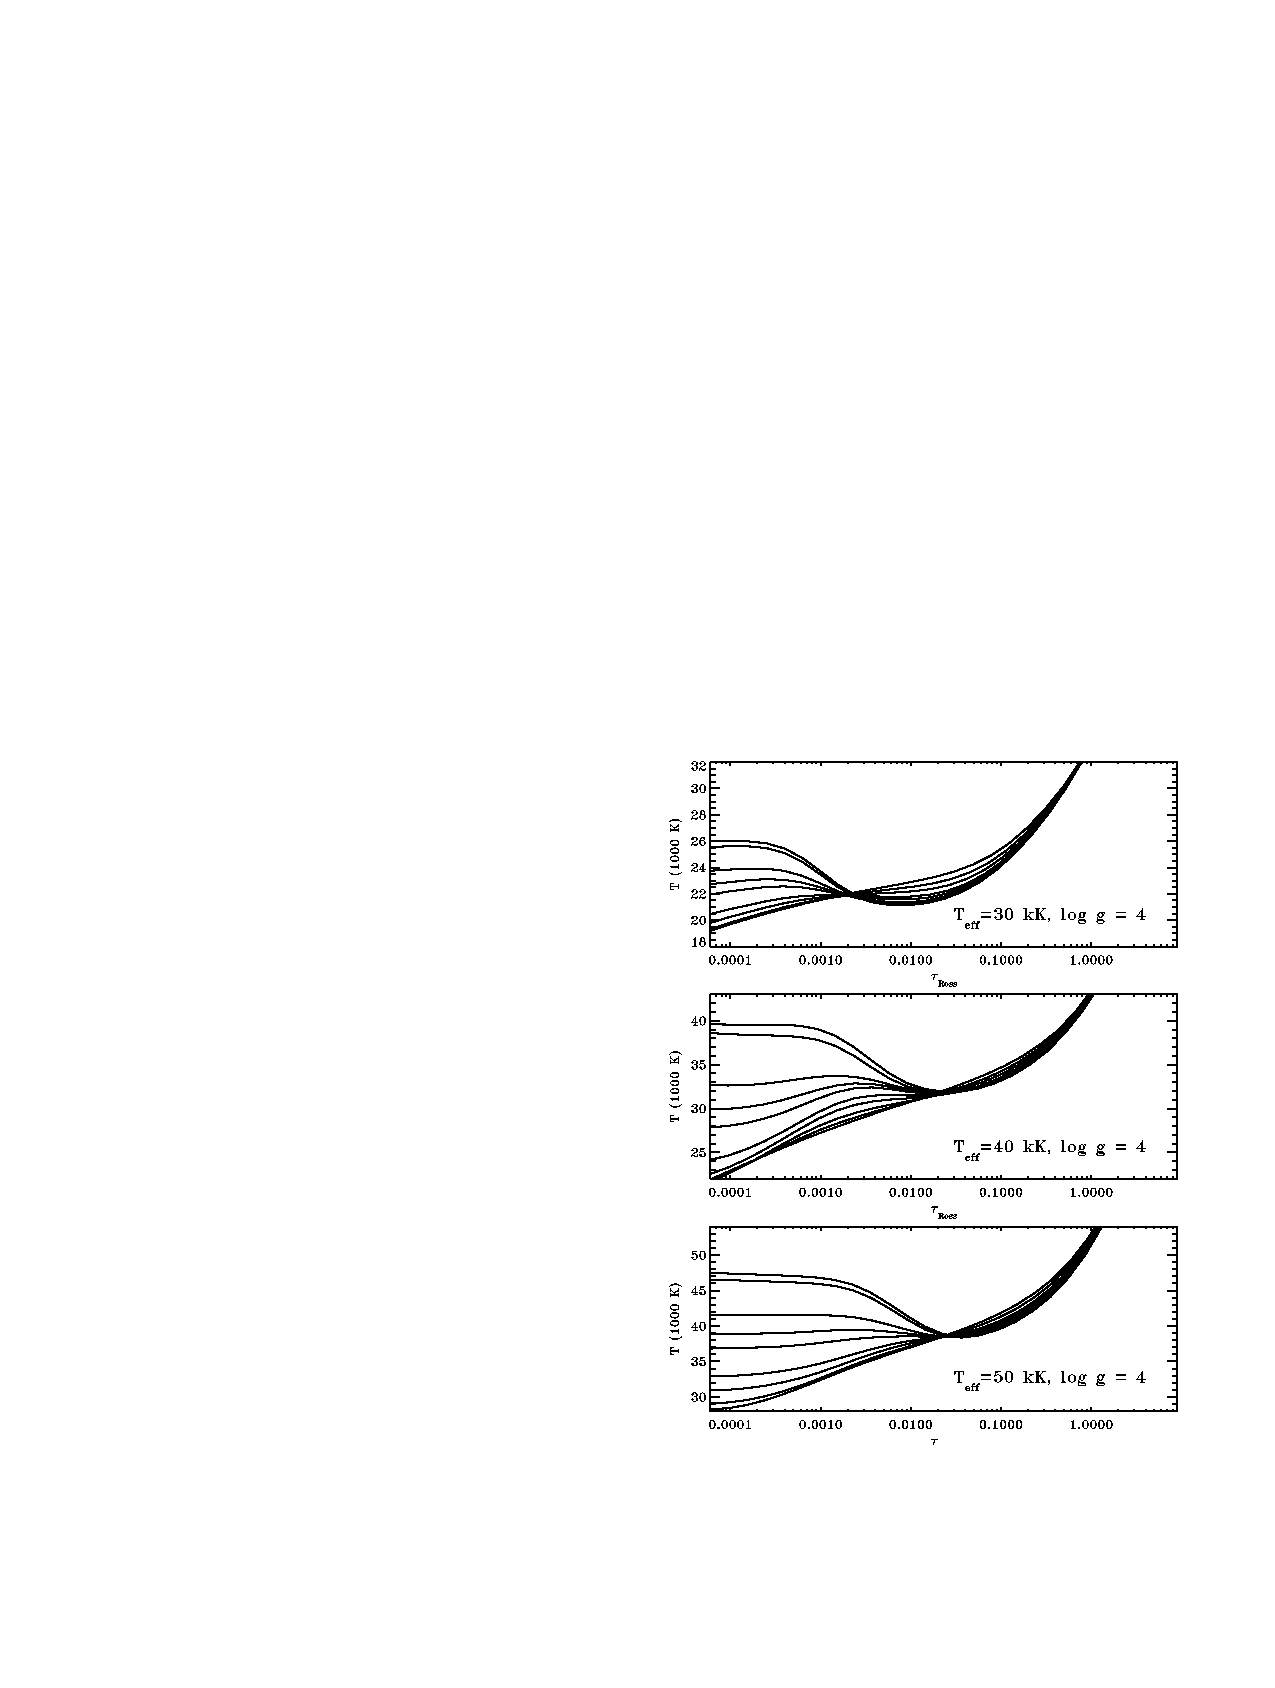
\includegraphics[width=\linewidth]{figures/lanz-hubeny-temperature.pdf}
\label{figure:lanz-hubeny-temperature}
\caption{Temperature as a function of optical depth in the NLTE models of Lanz \& Hubeny (2003). Three effective temperatures and ten metallicities are shown. In each case, the surface gravity is log g = 4.0. The metalicites range from metal-free to twice solar. At each effective temperature, the metal-free models have the highest surface temperature and the solar metallicity models have  the second lowest surface temperatures.}
\end{figure}

One would expect that the change in temperature would cause a change in the ionization fraction, in the sense that hotter temperatures would favor higher degrees of ionization. This is certainly the case, but there is a second effect that is a pure NLTE effect. Figure \ref{figure:lanz-hubeny-ionization}
 compares the ionization fractions of helium and carbon in models with effective temperatures of 30,000 K, 40,000 K, and 50,000 K and solar metallicity. The solid lines show the ionization fractions from the NLTE models. The dashed lines show the ionization fraction calculated in LTE using the electron density and temperature taken from the NLTE models. One can see that the dominant ionization state behaves quite similarly in NLTE and LTE. However, there are important differences in the other states. We see that the ionization states that are lower than the dominant state are typically less common and ionization states that are higher than the dominant state are typically more common. For example, in the 30,000 K model, the dominant state of carbon is C III, and we see that C II is suppressed and C IV is enhanced with respect to LTE. This shift in ionization is attributable to the contribution of photo-ionization in these atmospheres. Ions can be photo-ionized by the intense radiation coming from hotter, deeper layers, but recombined with electrons at the local temperature. This imbalance shifts the ionization to higher states.

\begin{figure}
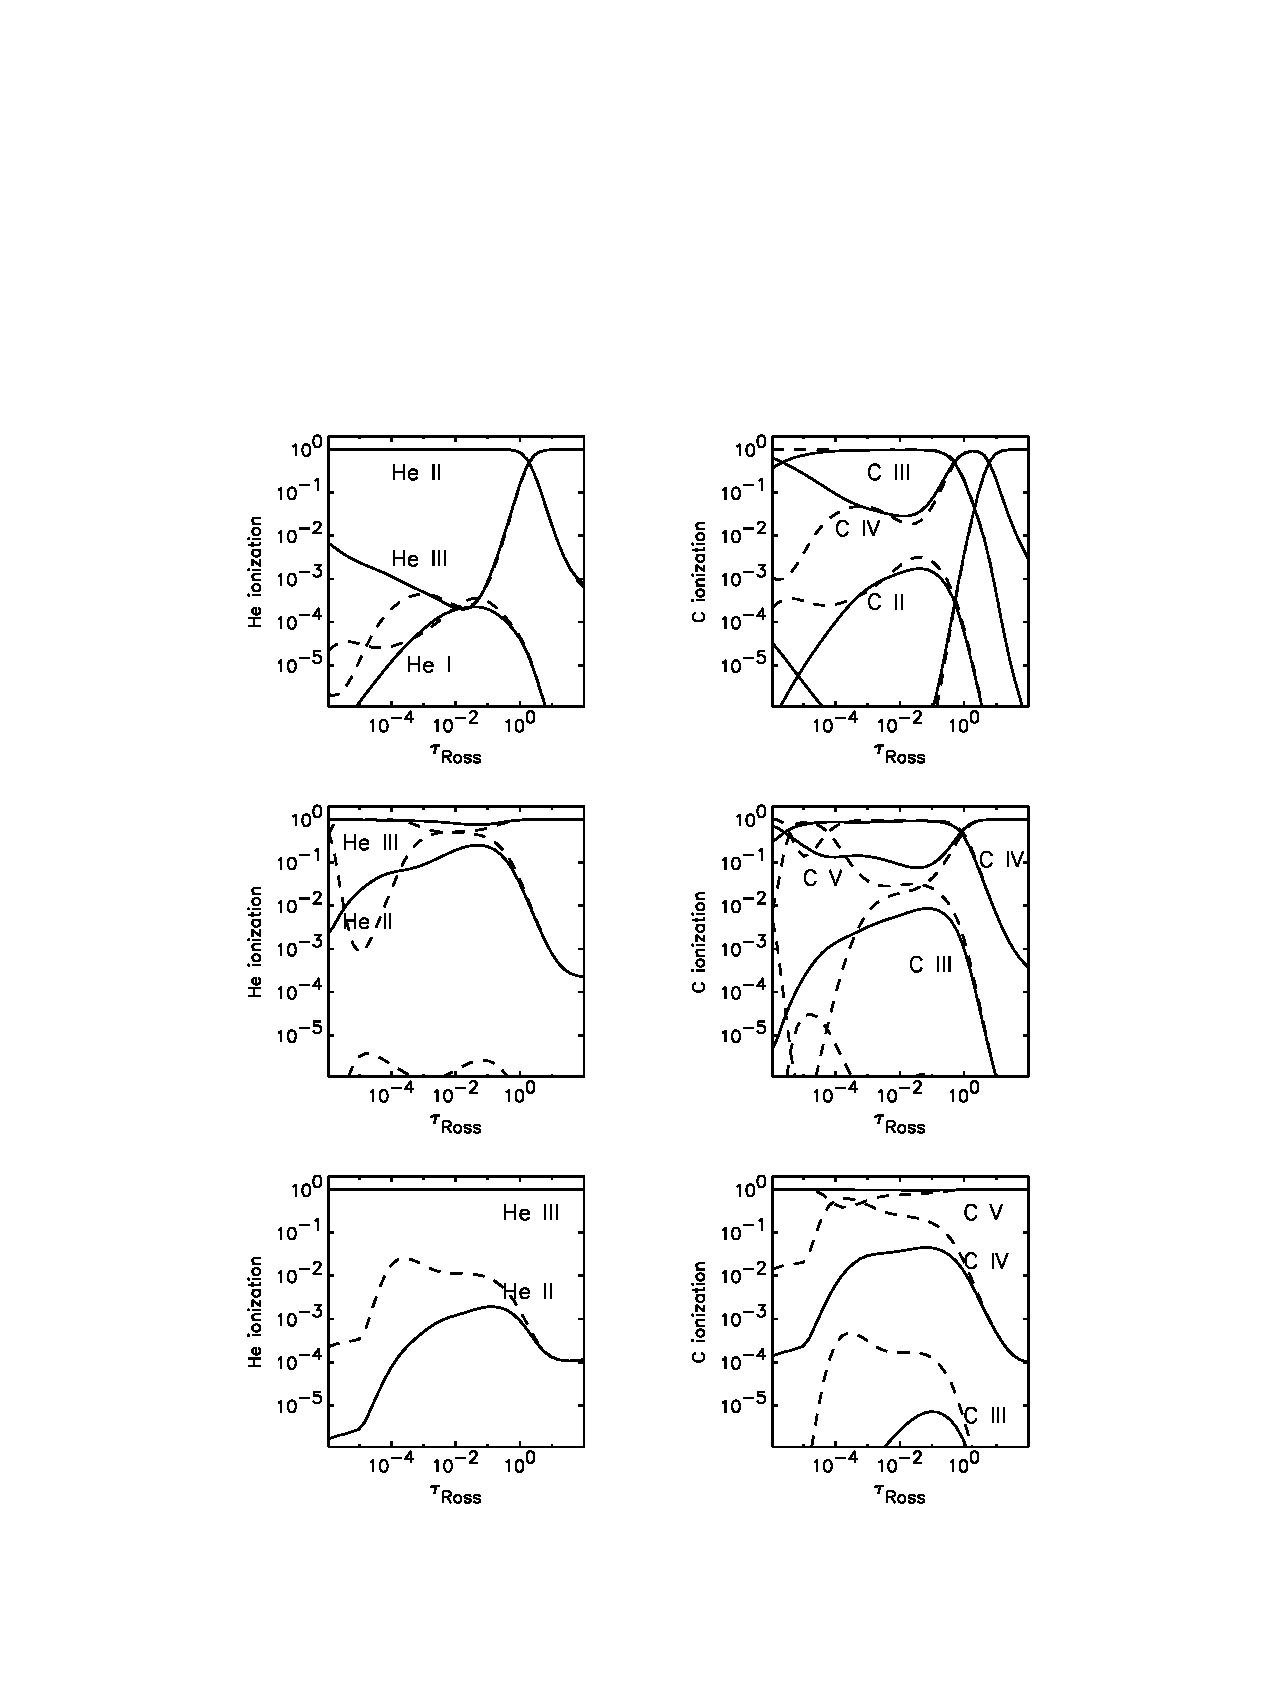
\includegraphics[width=\linewidth]{figures/lanz-hubeny-ionization.pdf}
\label{figure:lanz-hubeny-ionization}
\caption{Ionization fractions of helium and carbon as a function of optical depth in the NLTE models of Lanz \& Hubeny (2003). Three effective temperatures are shown. In each case, the surface gravity is log g = 4.0 and the metallicity is solar. The ionization fraction from the NLTE models are shown as solid lines. The ionization fraction in LTE calculated using the Saha distribution using the electron density and temperature from the NLTE model are shown as dashed lines.}
\end{figure}

The authors present a comparison of the emergent fluxes in their NLTE models and in the LTE models of Kurucz (1993). At low resolution in the optical and near-ultraviolet, the two sets of models are in relatively good agreement. However, the authors suggest that at the higher resolutions typically used to determine stellar parameters, their models are more reliable. The authors also consider the photon fluxes q0 and q1 in the H I (Lyman) and He I ionizing continua below 912 Å and 504 Å. They do not consider the photon flux q2 in the He II ionizing continuum below 228 Å as this is typically formed in the wind (Gabler, Kudritzki, \& Mendez 1991; A\&A, 245, 587). This is an example of a limitation of their hydrostatic models. The values of q0 calculated from their models and from LTE models were in systematic agreement, but individual models differed by factors of up to 1.5 higher or lower. However, the NLTE values of q1 were systematically higher by a factor of 1.8 compared to the LTE models, with individual models differing by up to a factor of 3. The value of q1 is important for models of H II regions.
The authors consider that, within the limitations of a plane-parallel atmosphere in radiative equilibrium, the most serious shortcomings in their models a crude treatment of collisional rates for forbidden transitions of iron and nickel and their neglect of higher states of light elements such as carbon.

\newslide

\subsection{Short \& Hauschildt (2005)}

Here we will consider the LTE and NLTE models of the Sun presented by Short \& Hauschildt (2005; ApJ, 618, 926). Their NLTE models are “full NLTE” models in which both the atmospheric structure and emergent flux are calculated under NLTE. In comparison, the earlier models of Allende Prieto, Hubeny, \& Lampard (2003; ApJ, 591, 1192) were "restricted NLTE" models, in which the atmospheric structure was calculated in LTE and only the emergent flux using NLTE.

The solar atmosphere is obviously cooler than the atmosphere of an O star and more species contribute to the structure and opacity. The models of Short \& Hauschildt include H, He, Li, C, N, O, Ne, Na, Mg, Al, Si, P, S, K, Ca, Ti, Mn, Fe, Co, and Ni, twice as many elements as in the O star models of Lanz \& Hubeny (2003).

These authors do not adopt "superlevels". Instead, they treat levels connected by relatively strong transitions (those with log gf greater than -3) in NLTE and all others in LTE (i.e., using the Boltzmann distribution with the local temperature and electron density). They treat a total of about 6500 levels in NLTE.

The authors begin by showing that the temperature differences between LTE and NLTE models are less than 250 K. The NLTE model is 200 K warmer close to the surface (above optical depths of 0.01) and 150 K cooler at the base of the photosphere (at optical depths above 10). These changes are much less than in the case of O stars, in which we observed changes of thousands of K. This is expected; LTE is a better approximation in the photosphere of the Sun because the radiation field is weaker and collisions are more dominant.

However, despite the similarity in temperature between the LTE and NLTE models, there are significant differences between the emergent fluxes in the UV. The reason for this is that Fe I provides significant opacity in the UV, although Fe II is the dominant ionization state. The NLTE model show enhanced ionization of Fe I resulting from photo-ionization from the hotter, deeper layers. As can be seen in Figure \ref{figure:short-hauschild-pressure}, this reduces the abundance of Fe I and lowers the opacity in the UV. 

\begin{figure}
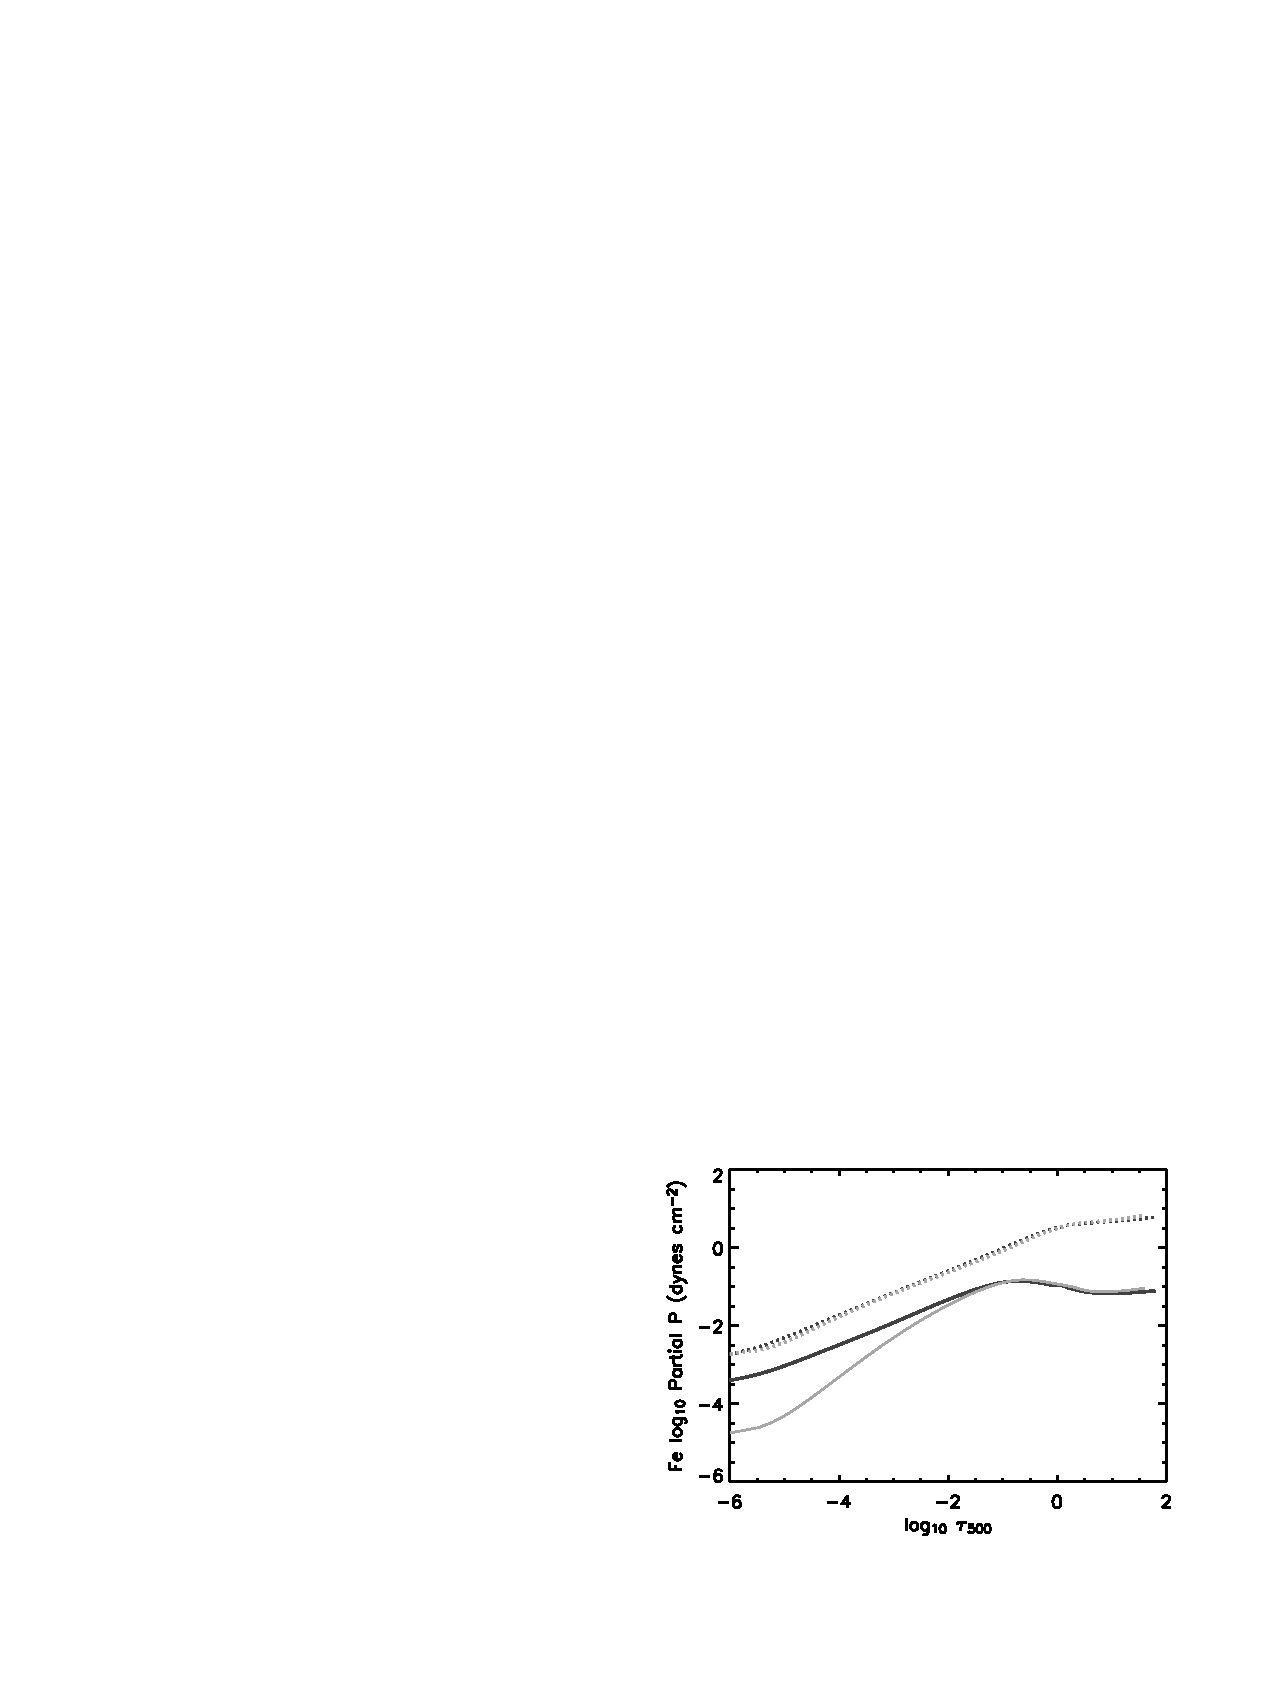
\includegraphics[width=\linewidth]{figures/short-hauschild-pressure.pdf}
\label{figure:short-hauschild-pressure}
\caption{Partial pressures of Fe I (solid lines) and Fe II (dotted lines) in the LTE (thick lines) and NLTE (thin lines) models of Short \& Hauschildt (2005).}
\end{figure}

The bad news is the NLTE model provides a worse fit to the observed flux than the LTE model. This is shown in Figure ref{figure:short-hauschild-flux}. In the UV, below about 4200 Å, the LTE model over-predicts the flux by about 10\% whereas the NLTE model over predicts the flux by about 30\%. The authors suggest that this “may indicate that the adoption of LTE masks some other inadequacy in the models”. They suggest that it is likely that there is a significant source of opacity that is still missing from the models.

\begin{figure}
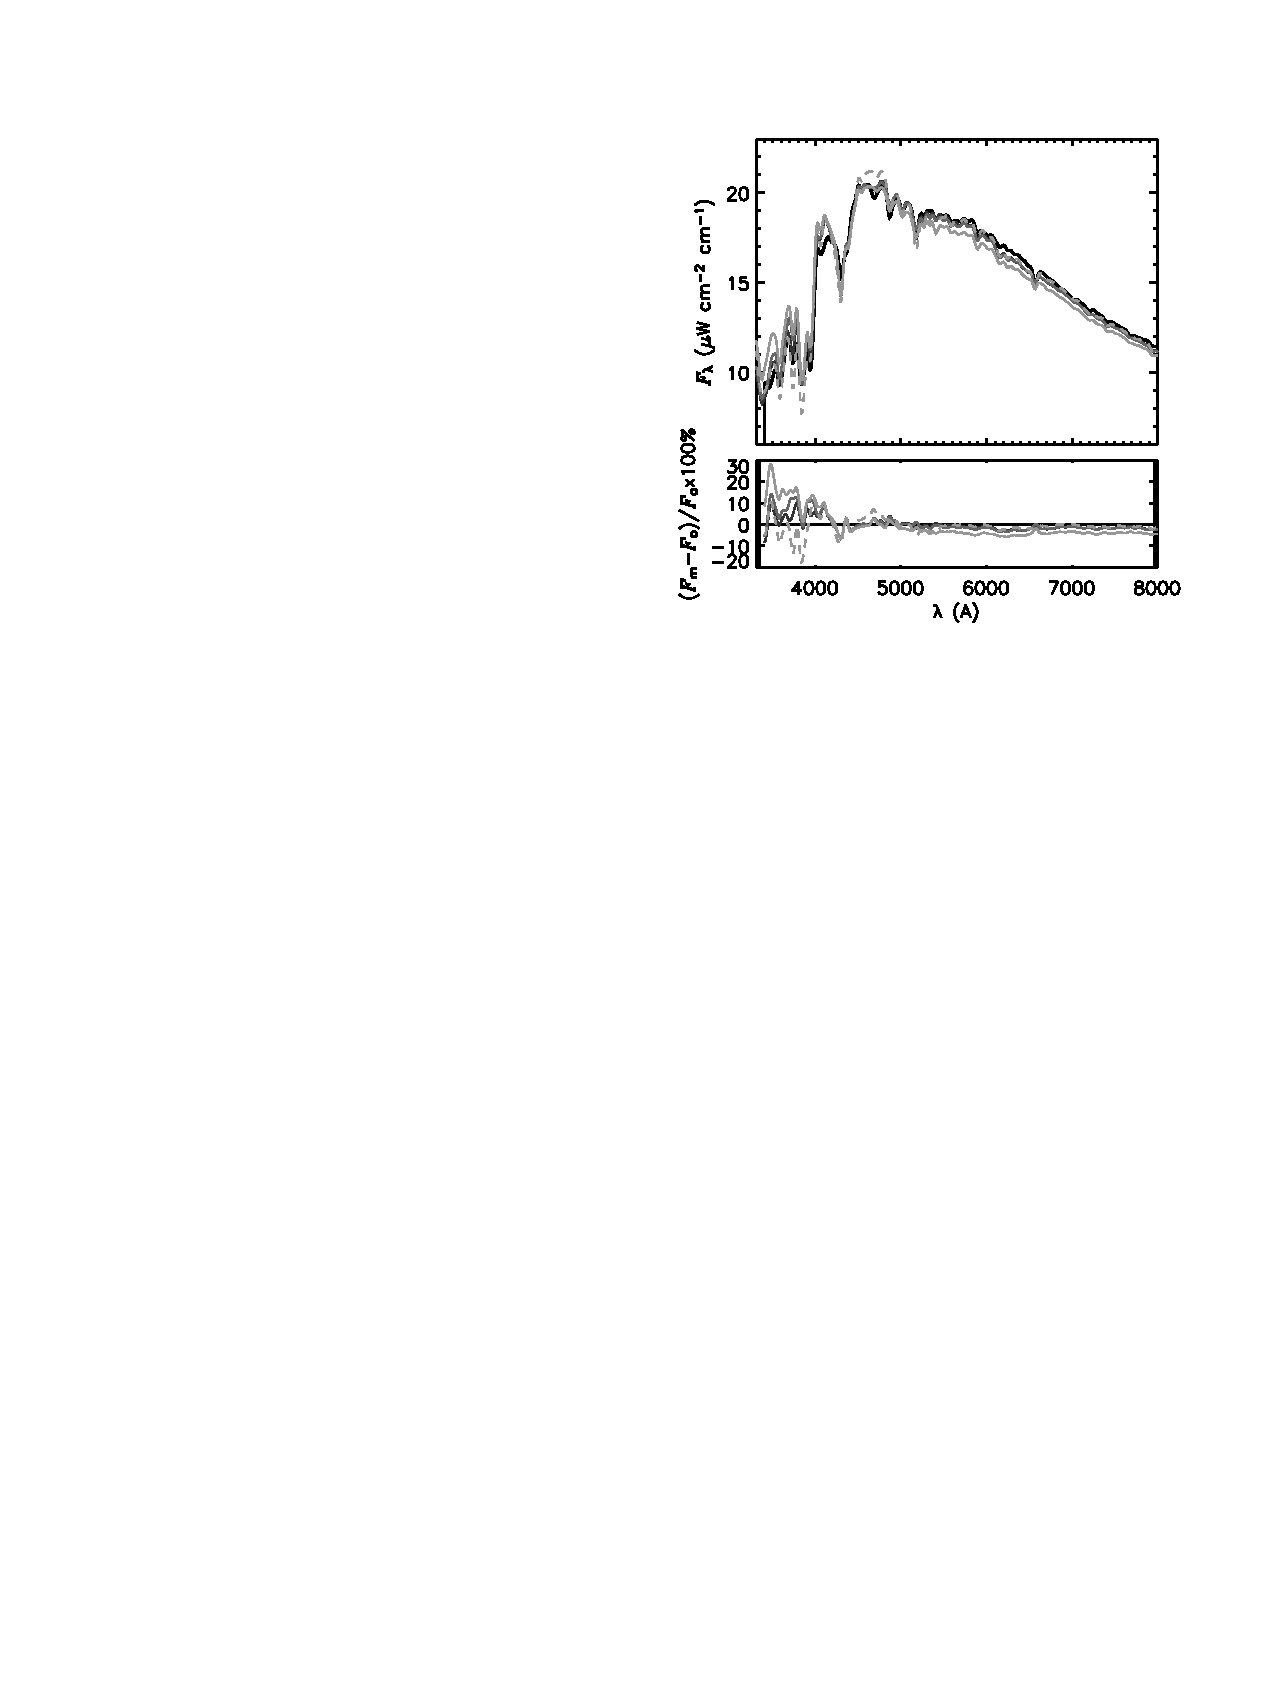
\includegraphics[width=\linewidth]{figures/short-hauschild-flux.pdf}
\label{figure:short-hauschild-flux}
\caption{Comparison of the absolute flux of the Sun measured by Neckel \& Labs (1984) and the LTE and NLTE models of Short \& Hauschildt (2005). The thick black line is the measured flux. The thin black line is the flux from the LTE model. The light gray line is the NLTE model. The lower panel shows the difference between the model fluxes and the observed flux.}
\end{figure}

\newslide

\subsection{Summary}

As we have seen, NLTE effects are important in stars as diverse as O stars and solar-type stars. However, we have also seen that NLTE models are not magically correct in all respects. They suffer from uncertainties in atomic data and from the omission of important physics such as winds, chromospheric heating, and inhomogeneities. Nevertheless, NLTE is an important step towards more realistic models.


